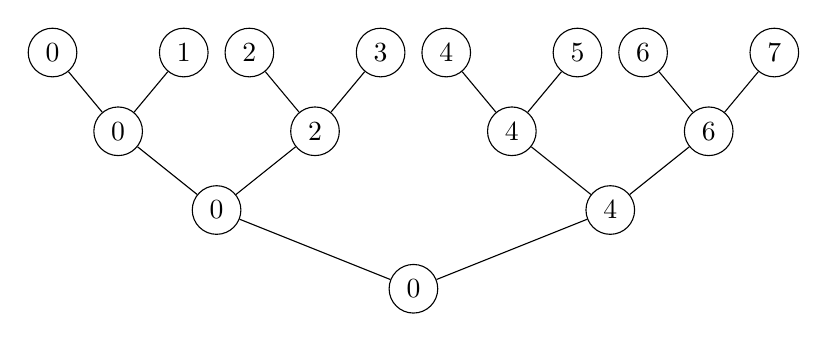
\begin{tikzpicture}[
        grow'=up,
        every node={
                style={
                        draw,align=center
                    }
            },
        level distance=1cm,
        level/.style={sibling distance=5cm/#1}
    ]
    \tikzset  {
        treenode/.style = {circle, draw=black, align=center, minimum size=0.5cm},
    }
    \node [treenode] {0}
    child {
            node [treenode] {0}
            child
                {
                    node [treenode] {0}
                    child {
                            node [treenode] {0}
                        }
                    child {
                            node [treenode] {1}
                        }
                }
            child
                {
                    node [treenode] {2}
                    child {
                            node [treenode] {2}
                        }
                    child {
                            node [treenode] {3}
                        }
                }
        }
    child {
            node [treenode] {4}
            child
                {
                    node [treenode] {4}
                    child {
                            node [treenode] {4}
                        }
                    child {
                            node [treenode] {5}
                        }
                }
            child
                {
                    node [treenode] {6}
                    child {
                            node [treenode] {6}
                        }
                    child {
                            node [treenode] {7}
                        }
                }
        }
    ;
\end{tikzpicture}
